\documentclass[12pt,letterpaper]{article}

\edef\origparind{\the\parindent}

\usepackage[utf8]{inputenc}
\usepackage[margin=1in]{geometry}
\usepackage{setspace}
\usepackage{blindtext}
\usepackage[T1]{fontenc}
\usepackage{amsmath}
\usepackage{times}
\usepackage{graphicx}
\usepackage{hyperref}
\usepackage[font=footnotesize]{caption}
\usepackage{relsize}
\usepackage{environ}
\usepackage[skip=0.5cm]{parskip}
\usepackage[sorting=none]{biblatex}
\usepackage{tikz}
\usepackage{pgfplots}
\usepackage{paralist}
\usepackage{amssymb}
\usepackage{listings}
\usepackage{color}

\usetikzlibrary{positioning}
\pgfplotsset{compat=1.16}

\parindent=\origparind\relax

% STUFF
\DeclareCaptionType{equ}[][]

\setstretch{1.4}

\makeatletter
\def\maketag@@@#1{\hbox{\m@th\normalfont\normalsize#1}}
\makeatother

\NewEnviron{EQUATIONS}{%
  \scalebox{1.25}{$\BODY$}
}

\addbibresource{main.bib}
% STUFF END

\title{\textbf{master's project notes}}
\date{}
\author{}

\begin{document}

% Title
\maketitle
\newpage 

% Table of contents
\tableofcontents
\newpage

%\section{Evaluation of NumPy vs CuPy in npstructures and BioNumpy}
To initiate exploration of what CuPy does well in comparison to NumPy, I am carefully benchmarking each step of the k-mer counting pipeline, going from an input fasta file of 20 million reads to the finished counter object, in order to fully understand which parts of the npstructures and BioNumpy code is lacking relative performance using both NumPy and CuPy as the backend array module.

This pipeline, as is performed in the BioNumpy library, can be abstracted into n parts: 
1) reading and formatting a chunk of reads from the input fasta file, resulting in a ragged-array containing a single read per row, where each base is represented as a single unsigned 8-bit integer. 
2) Converting the chunk of reads into a compact bit-array representation, only using 2 bits per base. 
3) retrieving each 31-mer from the bit-array and representing each 31-mer as a 64-bit integer. 
4) ...

\subsection{Reading fasta file and creating chunks of reads}
Practically all of the time spent when preparing each chunk in the chunk generator is spent in OneLineBuffer\textsc{'}s get\_data() method.
Further examining this method revealed that the entire process of looping through each chunk (with the chunk size set to the default 5M bytes), spent only 3.4 of 13.8 total seconds in a 

%\section{Examining counter implementations}
\subsection{The npstructures counter object}
The counter object found in the npstructures package is a specialized hashtable used for counting frequencies of unique 64-bit data values.
The original npstructures counter object and its underlying hashtable are implemented in Python, and therefore rely heavily on NumPy to perform its underlying functionalities efficiently.
Describe the npstructures counter object ...

% Overview of the npstructures.Counter object
Diagrams?

\subsection{CUDA counter}
One of the primary issues with the npstructures counter object is that its implementation is constrained by the functionalities provided by NumPy for good performance.
This results in a sequence of, perhaps unnecessary, array operations for initialization, counting and lookups.
In an attempt to mitigate this, I implemented a simpler and more straightforward counter object in CUDA and used the pybind11 library to create Python bindings for the implementation as to create a drop-in replacement for the npstructures counter object.

Describe the CUDA counter implementation ...

%\begin{figure}[h!]\label{figure:gpu-system}
%\begin{center}
%\begin{tikzpicture}

%  \node at(0,2)[rectangle,draw](cpu){CPU};
%  \node at(0,0)[rectangle,draw](cpuram){RAM};
%  \node at(5,2)[rectangle,draw](gpu){dGPU};
%  \node at(5,0)[rectangle,draw](gpuram){Device RAM};

%  \draw [-stealth](cpu) -- (cpuram);
%  \draw [-stealth](gpu) -- (gpuram);
%  \draw [stealth-stealth](cpuram) -- (gpuram);

%  \node at(2.5,0.3){\smaller PCIe};
%  \node at(0,3){\small Host};
%  \node at(5,3){\small Device};
%  \node at(0,1)[rectangle,draw,minimum width=2cm,minimum height=3cm](hostunit){};
%  \node at(5,1)[rectangle,draw,minimum width=3cm,minimum height=3cm](deviceunit){};

%\end{tikzpicture}
%\caption{A typical CPU and dGPU setup.}
%\end{center}
%\end{figure}

\subsection{Performance comparison}
...

Comparison between different hashtable capacity sizes for the CUDA hashtable implementation. We expect faster initialization, counting and lookup when the capacity is larger. 
The following bar chart show the time spent processing counts in the hashtable for 20 million reads of 150 bases.
The counter object was initialized with 20 million unique kmers as keys, and the fasta file containing the reads was in chunks of 10 million bytes using BioNumPy.
Since the counter object was initialized with 20 million keys, the theoretical smallest possible capacity of the hashtable was 20 million slots.
The tests benchmarked the total time spent waiting for the count call, summarized from all the chunks making up the 20 million reads.

\begin{figure}[ht!]\label{figure:cuht-capacity}
\begin{center}
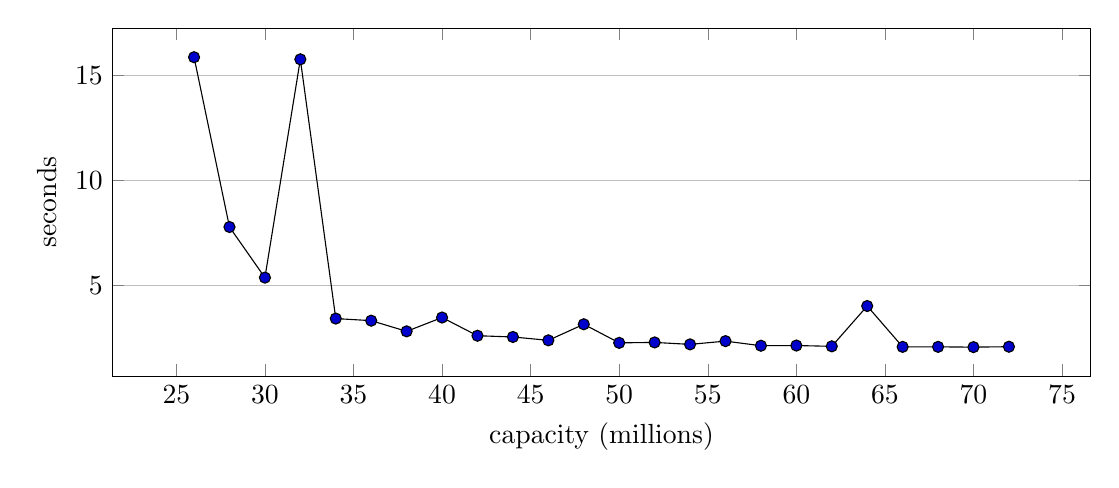
\begin{tikzpicture}
 
\begin{axis} [
  ymajorgrids = true,
  ylabel = {seconds},
  xlabel = {capacity (millions)},
  %bar width = 0.4cm,
  %ybar,
  height = 6cm,
  width = 14cm
]
\addplot+[black] coordinates {
    (26,15.857)
    (28,7.788)
    (30,5.383)
    (32,15.757)
    (34,3.436)
    (36,3.337)
    (38,2.829)
    (40,3.486)
    (42,2.621)
    (44,2.562)
    (46,2.402)
    (48,3.166)
    (50,2.282)
    (52,2.303)
    (54,2.21)
    (56,2.364)
    (58,2.146)
    (60,2.155)
    (62,2.117)
    (64,4.033)
    (66,2.092)
    (68,2.092)
    (70,2.079)
    (72,2.099)
};
%\addplot+[red] coordinates {
    %(70,2.079)
%};
\end{axis}
 
\end{tikzpicture}
\caption{The total time spent waiting for the count calls when counting 20 million reads of 150 bases each. As expected, the tradeoff between memory and efficiency becomes apparent as larger capacities result in faster counting times. Although we quickly reach a point of dimishing returns, we see small improvements all the way up to a capacity of 70 million slots, with a capacity of 70 million slots spending a total of 2.079 seconds counting 20 million reads. The benchmark was only ran from 26 million up to 72 million slots. Time consumption grew exponentially with smaller capacities than 26 million for this counter of 20 million keys.}
\end{center}
\end{figure}

...

\begin{figure}[ht!]\label{figure:nps-vs-cu}
\begin{center}
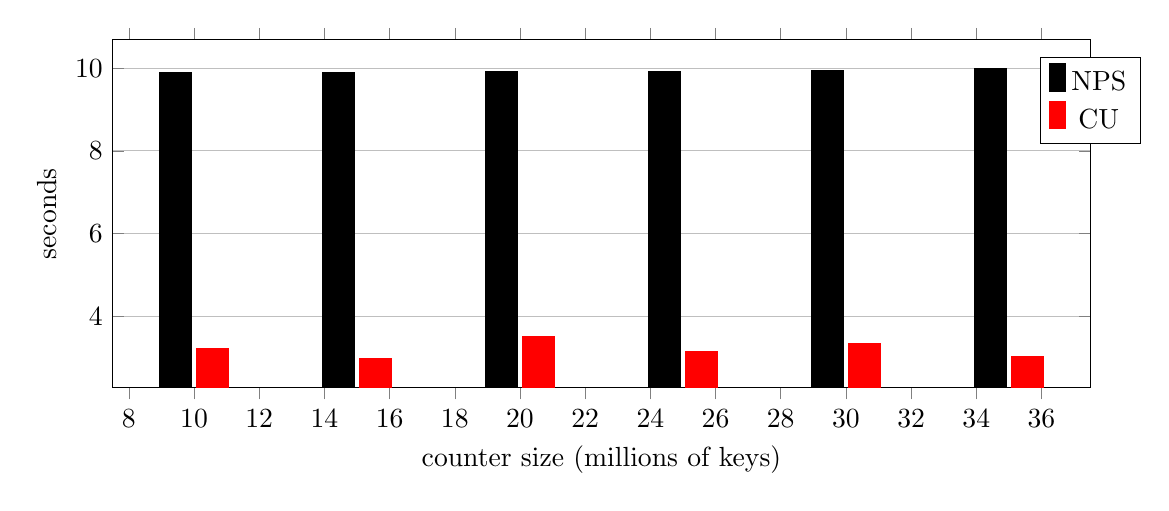
\begin{tikzpicture}
 
\begin{axis} [
  ymajorgrids = true,
  xlabel = {counter size (millions of keys)},
  ylabel = {seconds},
  bar width = 0.4cm,
  ybar,
  height = 6cm,
  width = 14cm,
  legend style = {at={(1,0.95)}, anchor=north},
  legend image code/.code={\draw [#1] (0cm,-0.1cm) rectangle (0.2cm,0.25cm);},
]
\addplot+[black] coordinates {
    (10,9.882)
    (15,9.896)
    (20,9.927)
    (25,9.91)
    (30,9.936)
    (35,9.985)
};
\addplot+[red] coordinates {
    (10,3.22)
    (15,2.975)
    (20,3.514)
    (25,3.147)
    (30,3.339)
    (35,3.027)
};
\legend{NPS,CU}
\end{axis}
 
\end{tikzpicture}
\caption{CUDA counter uses a capacity factor of 2.0.}
\end{center}
\end{figure}

\section{Fast poisson logpmf}
\subsection{The implementations}
The poisson logpmf is something aaaa

We have four different implementations performing (poisson logpmf?) ... :


\definecolor{keywordclr}{rgb}{0,0,1}
\definecolor{stringclr}{rgb}{0.75,0.15,0.15}
\definecolor{commentclr}{rgb}{0.5,0.5,0.5}

\lstset{frame=tb,
  language=Python,
  aboveskip=3mm,
  belowskip=3mm,
  showstringspaces=false,
  columns=flexible,
  basicstyle={\small\ttfamily},
  numbers=left,
  numberstyle=\smaller\color{commentclr},
  keywordstyle=\color{keywordclr},
  commentstyle=\color{commentclr},
  stringstyle=\color{stringclr},
  breaklines=true,
  breakatwhitespace=true,
  tabsize=4
}

The first implementation we consider is the implementation provided by the SciPy \cite{SciPy}
\begin{lstlisting}
from scipy.stats import poisson

def poisson_logpmf(k, r):
    return poisson.logpmf(k, r)
\end{lstlisting}

\pgfplotsset{
  compat=newest,
  xlabel near ticks,
  ylabel near ticks
}

\begin{figure}[ht!]\label{figure:poisson_logpmf_performance}
\begin{center}
  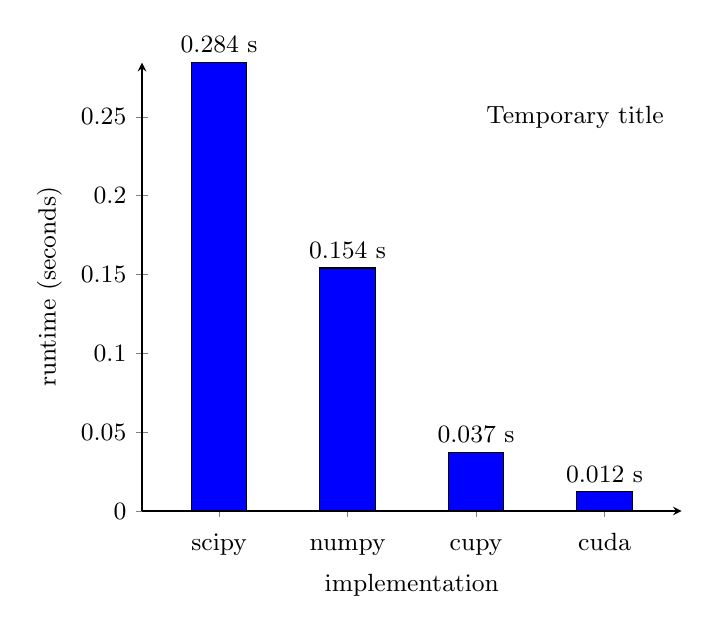
\begin{tikzpicture}[font=\small]

  \node at(5.5,5)(title){Temporary title};
 
\

\begin{axis} [
  ylabel={runtime (seconds)},
  xlabel={implementation},
  ybar,
  bar width=20pt,
  ymin=0,
  %ytick=\empty,
  xtick=data,
  axis x line=bottom,
  axis y line=left,
  enlarge x limits=0.2,
  symbolic x coords={scipy, numpy, cupy, cuda},
  xticklabel style={anchor=base, yshift=-\baselineskip},
  /pgf/number format/.cd,fixed,precision=3,
  nodes near coords={\pgfmathprintnumber{\pgfplotspointmeta} s},
]

\addplot[fill=blue] coordinates {
    (scipy, 0.2843504619598389)
    (numpy, 0.15413585186004639)
    (cupy, 0.037178173065185546)
    (cuda, 0.012188527584075928)
};

%\legend{SciPy, NumPy, CuPy, CUDA}
\end{axis}
 
\end{tikzpicture}
\caption{Temporary caption.}
\end{center}
\end{figure}

Some more text.


\newpage
\printbibliography

\end{document}
